\documentclass[a4paper,12pt,article]{memoir}
\usepackage{amsmath}
\usepackage{amssymb}
\usepackage{mathspec}
\usepackage{xltxtra}
\usepackage{polyglossia}
\usepackage{siunitx,cancel,graphicx}
\usepackage{enumitem}
\usepackage{hyperref,graphicx}
\usepackage{icomma}
\usepackage{float}
\usepackage{mleftright}

\usepackage{listings}
\usepackage{color}

\usepackage[
backend=biber,
style=numeric,
citestyle=numeric,
sorting=none
]{biblatex}
\addbibresource{resources.bib}


\definecolor{MyDarkGreen}{rgb}{0.0,0.4,0.0}
\definecolor{Blue}{rgb}{0.0,0.0,1.0}
\definecolor{Purple}{rgb}{1.0,0.0,1.0}

\lstset{language=c++,
                basicstyle=\ttfamily,
                keywordstyle=\color{blue}\ttfamily,
                stringstyle=\color{red}\ttfamily,
                commentstyle=\color{green}\ttfamily,
                morecomment=[l][\color{magenta}]{\#},
                breaklines=true
}

\setdefaultlanguage{english}

\defaultfontfeatures{Scale=MatchLowercase,Mapping=tex-text}
%\setmainfont[Numbers=Lowercase]{Minion Pro}
%\setsansfont[Numbers=Lowercase]{Myriad Pro}
%\setmonofont{Menlo}
%\setmathsfont(Digits,Latin,Greek)[Numbers={Lining,Proportional}]{Minion Pro}

\sisetup{%
  output-decimal-marker = {,},
  per-mode = symbol,
  %round-mode = places,
  %round-precision = 5
}



\setlrmarginsandblock{2.5cm}{2.5cm}{*}
\setulmarginsandblock{1.5cm}{2cm}{*}
\checkandfixthelayout

\setlength{\parindent}{2em}
\setlength{\parskip}{0pt}

\newcommand{\f}{\fancybreak}

\DeclareSIUnit \electronvolt {\ensuremath{eV}}

\newcommand{\mvec}[2]{
\ensuremath{\left(
\begin{array}{c}
#1\\
#2\\
\end{array}
\right)}
}

\title{Working with the Bose-Hubbard model on a flat rectangular lattice with the Bose-Hubbard model }
\date{2023} %

\begin{document}

\maketitle

In this document, I go through my code for finding the lowest few Eigenstates of a number of particles, on a rectangular, using the Bose-Hubbard model with only closest neighbor interactions. At the current state, the code can in principle work with a lattice with up to 64 sites such as 8x8 (but in practice, that is computationally completely unreasonable, with more than 2 particles).


\section{The Hamiltonian, theoretically}
The free Hamiltonian is a simplified version of the Bose Hubbard model (Equation 9 in \cite{Nielsen2021}, with $t(z_j,z_k)=0$ for not nearest neighbour)):

\begin{equation}
H_0=\sum_{j\neq k} t(z_j,z_k)\hat{a}_j^\dagger \hat{a_k}.
\end{equation}


Where $\hat{a}_j$ is the annihilation operator for a boson on lattice site $j$ at position $z$, where at most one boson can exist on any site. Being hermitian, $t(z_j,z_k)=t^*(z_j,z_k)$. Furthermore \cite{Nielsen2021} quotes $t(z_j,z_k)$ as:

\begin{equation}
t(z_j,z_k)= (-1)^{\Re(z_j-z_k)+\Im(z_j-z_k)+\Re(z_j-z_k)\Im(z_j-z_k)}t_0 \exp^{-(\pi/2)(1-\phi)|z_j-z_k|^2}\exp(-i\pi\phi[\Re(z_j)+\Re(z_k)]\Im(z_j-z_k)).
\end{equation}

For some constant $t_0$ and $\phi$. Where the real and imaginary parts of $z_j$ is the $x$ and $y$ location of the lattice cite. This is not entirely what I use. Firstly since we only consider nearest neigbours the first two terms are constant and can be folded into $t_0$. Secondly, the above equation makes the phase $0$ if $\Im(z_j-z_k)=\Delta y =0$ and proportional to $x$ otherwise, as we discussed the phase being proportional to $y$ if going between neighbours at the same height, and $0$ if going between neighbours at the same $x$, I pick:

\begin{equation}
t(z_j,z_k)= t_0 \exp(-i\pi\phi[\Re(z_j)+\Re(z_k)]\Im(z_j-z_k)/2)= \begin{cases}t_0\exp(i0) & \Delta y = 1, \Delta x=0  \\ t_0\exp(iy) & \Delta y = 0, \Delta x=1\\ 0 & \mathrm{otherwise} \end{cases}.
\end{equation}

Where I set $\phi=1$ and energy scale $t_0=1$. Furthermore a potential $U_j$ can be added to the Hamiltonian for each lattice site.

\begin{equation}
H=H_0+\sum_j U_j \hat{a}_j^\dagger\hat{a}_j.
\end{equation}

Finding the energy and Eigenstates is a matter of diagonalising the Hamiltonian, in the basis of the allowed states. The states can be written as $|n_0n_1\ldots n_{N_{s}} \rangle$ for $N_{s}$ sites with $n_j=0$ or $n_j=1$ hard-core bosons, where $\sum_j n_j=N$. So one state in a 4x2 lattice with 8 sites and 3 particles could for instance be $|1011000\rangle$ (In practice I will write $|n\rangle$ where $n$ is the unsigned integer corresponding to this state in little-endian notation). Exactly what $n_j$ refers to which site does not matter, in my case $n_0$ is the top left site, continuing in reading order.

The free Hamiltonian matrix between state $|n\rangle$ and $|m\rangle$ is then:

\begin{equation}
[H_0]_{nm}=\sum_{j,k\in\mathrm{neighbors}}  t(z_j,z_k) \langle n| \hat{a}_j^\dagger\hat{a}_k|m\rangle .
\end{equation}

But $ \langle n| \hat{a}_j^\dagger\hat{a}_k|m\rangle =0$ unless $|n\rangle$ and  $|m\rangle$ are identical, except the particles at site $j$ and $k$ are swapped, in that case $[H_0]_{nm}=t_0\exp(\mp \phi y)$ or $[H_0]_{nm}=t_0$.

The potential term simply adds the potential $U_j$ for each populated site in the state $|n\rangle$ to the diagonal:

\begin{equation}
[U]_{nn}=\sum_{j} u_j n_j.
\end{equation}

\section{Diagonalizing the hamiltonian, computationally}
The code is uploaded on Github \cite{code}, the Codes is tested on Arch-Linux and Debian, and requires the armadillo library and the gcc compiler to be installed already. It has not been tested on Windows.

I have ended up using $c++$, using the Armadillo Library \cite{arma}. After comparing a number of options, I have found that this is the fastest, best documented and has all the features I want (it supports general complex matrices, which can be represented as sparse matrices, which I do find to be worthwhile when  looking only at nearest neighbours). While the numpy package for python works too, I personally strongly prefer $c$ or $c++$.

Actually finding all the states correctly and efficiently was an interesting computational challenge, but not one I will delve on here, suffice it to say that I represent each state is a 64 bit unsigned integer, and I have a recursive algorithm for generating all legal states \lstinline{void generate(vector<uint64_t>& states,uint64_t& N_states,uint64_t N_sites,uint64_t N_particles);} which generates a list of all legal states for a given number of sites and particles.

The example makefile creates two programs, the first \lstinline{debug_showstates.exe} simply generates a tsv file (tab-separated-values) with all the basic states of a particularly sized lattice with $N$ particles, this tsv file is in a format which can be plotted by the gnuplot file \lstinline{plot.gpi}. Note that both programs prints a log to the standard output (\lstinline{cout} in c++) and the data to the error channel (\lstinline{cerr} in c++), to save the data to a file, for instance run \lstinline{./debug_showstates.exe 3 5 1> log.txt 2> states.tsv}.

\fancybreak

The other program, \lstinline{lattice_states.exe}, finds the lowest 3 energy eigenstates on a lattice of a particular size with a pre-defined number of particles. It does this by first generating all states $|n\rangle$, then looping through all states and all the states $|m\rangle$ which are at most one swap of a particle away, adding the contribution from this swap to $H_{nm}$ (in practice we only loop through swaps where $n<m$, and use the fact that the Hamiltonian is Hermitian), while also adding the potential at each occupied site in $|n\rangle$ to $H_{nn}$.

As things stand now, the potential is hard-coded, but it should be relatively simply to load that from an external file.

Finding the lowest 3 eigenstates is then a matter of writing:

\begin{lstlisting}
    //Somewhere to put the eigenvalues and vectors
    cx_vec eigval;
    cx_mat eigvec;

    //Here we get N_states eigenstates, we will only want to print the 3 lowest, so sort them in ascending order
    //eigs_gen means [eig]envalues of [s]parse [gen]eral (i.e. need not be square) matrix
    eigs_gen( eigval, eigvec, H, 3, "sr");//3,sr= 3 eigenvalues with smallest real part of the eigenvalues, hopefully the eigenvalues are REAL, but the function does not know that
\end{lstlisting}

As the armadillo library does not know that the Hamiltonian is hermitian, the eigenvalue returned is a complex number, but the imaginary part is always 0 (something the program automatically verifies in the end).

The eigenvector is the list of coefficients $c_0,c_1\ldots c_{N_s}$ specifying how much the eigenstate $|\phi\rangle$ is in any of the individual states $\sum_{n\in \mathrm{states}} c_n |n\rangle$.

To illustrate these eigenstates, the program generates a tsv file, which the gnuplot program \lstinline{plot1.gpi} can plot, showing the average number of particles in a particular site $\langle\phi|\hat{a}_j^\dagger \hat{a}_j|\phi \rangle=\sum_{n\in \mathrm{states}} c_n^2 n_j$.

In Figure \ref{fig:A} I shows the three lowest eigenstates for a 4 by 6 lattice with 8 particles with no applied potential, while \ref{fig:B} shows the same with a potential $-1$ at site (2,3) (counting from top-left, starting at index 0, it is very clear where the potential has been put). This size lattice with this number of particles takes around 10 minutes to calculate.

\begin{figure}
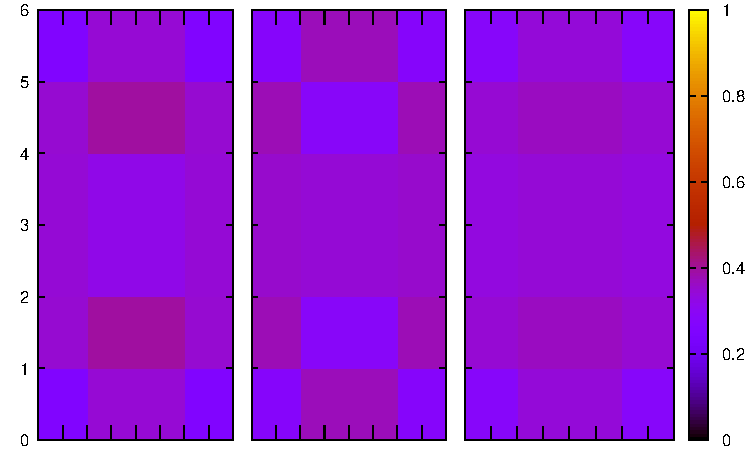
\includegraphics[width=\linewidth]{eigenstates.pdf}
\caption{The lowest three eigenstates (from left to right) of the example lattice, with no added potential.}
\label{fig:A}
\end{figure}


\begin{figure}
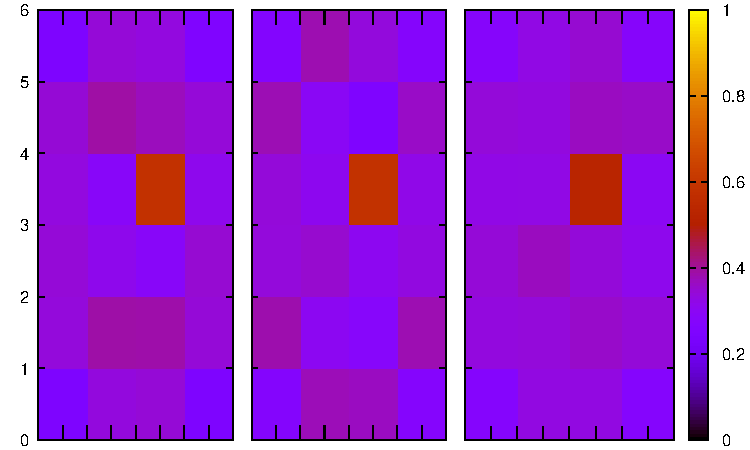
\includegraphics[width=\linewidth]{eigenstates_potential.pdf}
\caption{The lowest three eigenstates (from left to right) of the example lattice, with an arbitrary potential of -1 at the site 2,3).}
\label{fig:B}
\end{figure}

\printbibliography

\end{document}


